\documentclass[11pt]{article} % use larger type; default would be 10pt

\usepackage[slovene]{babel}
\usepackage[utf8]{inputenc}
\usepackage[T1]{fontenc}

\usepackage{amsmath}
\usepackage{amsthm}
\usepackage{amsfonts}
\usepackage{url}
\usepackage{graphicx}
\usepackage{enumerate}
\usepackage{caption}


\renewcommand\thesection{}
\renewcommand\thesubsection{\thesection \alph{subsection})}


\begin{document}
\begin{titlepage}
\centering
{\scshape\LARGE Fakulteta za matematiko in fiziko \par}
\vspace{1cm}
{\scshape\Large Iterativne numerične metode v lienarni algebri\par}
\vspace{1.5cm}
{\huge\bfseries 2.domača naloga\par}
\vspace{2cm}
{\Large\itshape Miha Avsec\par}
\vfill

\vfill

% Bottom of the page
{\large \today\par}
\end{titlepage}

Naloga je bila samostojno reševana s programom Matlab 2016a.

\section{1.naloga}

Množenje z matriko A implementiramo tako, da računamo produkt
$$Ax = \alpha Qx + 1/ne(d^tx) + (1-\alpha)1/nee^{T}x.$$
Na ta način ne potrebujemo polne matrike A, da bi izračunali produkt. Dominantne lastne vrednosti izračunamo s pomočjo potenčne in Arnoldijeve metode, ki smo jih implementirali na vajah.
Opazimo, da so ne glede na izbiro parametra $\alpha$ dominantne lastne vrednosti vedno $1$. Ne potenčna ne arnoldijeva metoda ne skonvergirata niti do natančnosti $10^{-3}$ po $150$ korakih. Vidimo, da pri Arnoldijevi metodi potrebujemo manj korakov, a je le ta počasnejša. Najbolj natančna in ekonomična pa je vgrajena matlabova metoda.

\section{2.naloga}

Območje $(0,3)\times(0,3)$ skrčimo na $(0,1)\times(0,1)$ tako, da $(0,1)\times(0,1)$ razdelimo na $9$ delov. V vsakem delu posebaj naredimo mrežo z $n$ točkami. To je ekvivalentno temu, da imamo v notranjosti $n-2$ točk na robu pa $2$ točki. Ko zlepimo vseh 9 kosov skupaj dobimo mrežo, ki ima v vsaki smeri $3n-2$ delilnih točk, ker se v notranjih na robu odsekov $(i,i+1)\times(j,j+1)$ točke ujemajo. Funkciji lik1(n) in lik2(n) tako vrneta matriki oštevilčenih točk velikosti $(3n-2)^2$. S pomočjo funkcije delsq potem rešimo diferencialni enačbi. Pri primerjavi najmanjših lastnih vrednosti vidimo da se le te razlikujejo za manj kot $10^{-6}$.
\newpage
\begin{centering}
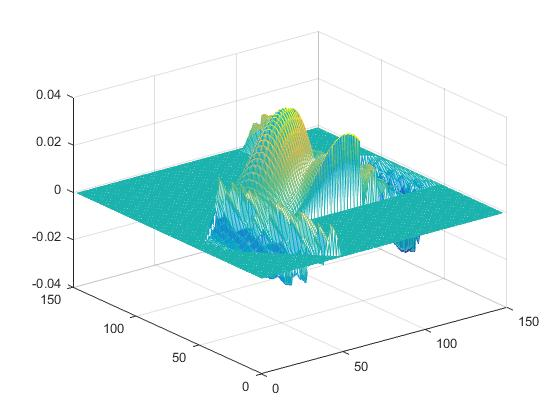
\includegraphics[scale=0.4]{lastna1}
\captionof{figure}{Lastna funkcija pri 5 najmanjši lastni vrednosti za lik1.}
\end{centering}

\begin{centering}
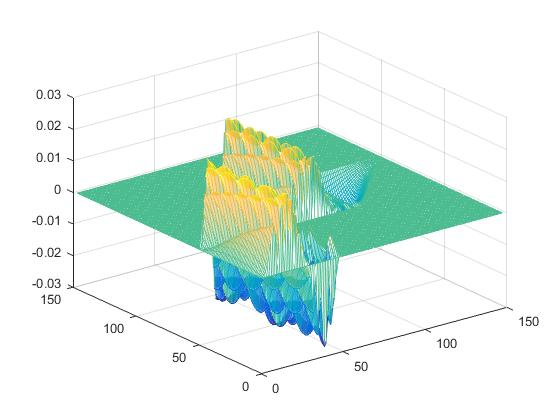
\includegraphics[scale=0.4]{lastna2}
\captionof{figure}{Lastna funkcija pri 5 najmanjši lastni vrednosti za lik2.}
\end{centering}

\newpage
\section{3.naloga}
Matriko A zapišemo kot incidenčno matriko povezav, kjer $(i,j)-ti$ element pomeni verjetnost prehoda iz $i-tega$ v $j-to$ vozlišče. Pri čemer so vozlišča urejena v stolpcu na naslednji način
$$(0,0),\ldots, (0,m-1), (1,0), \ldots, (1,m-2), \ldots$$
Pri $m=10$ kot rešitev tako dobimo največjo verjetnost $0.9$.

\begin{table}[!htbp]
\centering
\begin{tabular}{llll}
i-koordinata & j-koordinata & i-kordinata kamor gremo & j-koordinata kamor gremo \\
0            & 9            & 0                       & 8                        \\
9            & 0            & 8                       & 0                       
\end{tabular}
\end{table}

Pri $m=100$ kot rešitev tako dobimo največjo verjetnost $0.99$.


\begin{table}[!htbp]
\centering
\begin{tabular}{llll}
i-koordinata & j-koordinata & i-kordinata kamor gremo & j-koordinata kamor gremo \\
0            & 99            & 0                       & 98                        \\
99            & 0            & 98                       & 0                       
\end{tabular}
\end{table}

Pri $m=1000$ kot rešitev tako dobimo največjo verjetnost $0.999$.

\begin{table}[!htbp]
\centering
\begin{tabular}{llll}
i-koordinata & j-koordinata & i-kordinata kamor gremo & j-koordinata kamor gremo \\
0            & 999            & 0                       & 998                        \\
999            & 0            & 998                       & 0                       
\end{tabular}
\end{table}

Opazimo, da je največja verjetnost prehoda ravno v levem zgornjem in desnem spodnjem kotu.

\begin{centering}
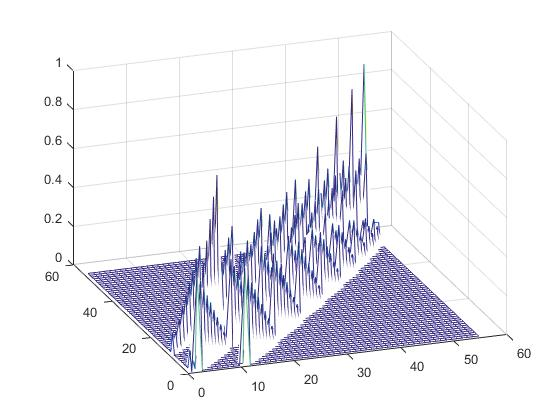
\includegraphics[scale=0.4]{G1}
\captionof{figure}{Graf verjetnosti prehoda iz posameznih točk za m=10.}
\end{centering}

\section{4.naloga}

Jacobijevom matriko generiramo tako, da najprej izračunamo vse odvode, ki so različni od $0$. Za u so to le odvodi po $u_{i,j},u_{i+1,j},u_{i-1,j},u_{i,j-1},u_{i,j+1},v_{i,j}$. Podobno pride tudi za v. Prav tako opazimo, da je Jacobijeva matrika brez naddiagonale in poddiagonale v resnici bločna matrika z bloki velikosti $2n$. Zato zgeneriramo posamezen blok, ki ga potemo vstavimo na prava mesta v matriki. Na koncu pa dodamo še obe zunanji diagonali, ki imata prav tako iste elemente, ki se ponavljajo. Nato naredimo funkcijo, ki v odvisnosti od parametra $L$ generira Jacobijevo matriko in še funkcijo, ki vrne $1$, če je največja realna lastna vrednost matrike, ki jo podamo kot argument, večja kot $0$ in $-1$ sicer. Nato na kompoziciji teh dveh funkcij poženemo bisekcijo. Kot rešitev dobimo vrednost $L=0.7236$.  
\end{document}

